\chapter{Used software infraestructure}

Before going deeper inside the software implementation made to solve the task of multiobject tracking it is necessary to introduce the software infraestructure needed to accomplish it. The name selected for the component or application built is \textit{dl-objecttracker}. This component is completely written in Python. In particular, the Python version used is the 2.7.12 mainly due to the compatibility with ROS. The component needs a set of parts for its perfect operation which, due to the nature of the task, the majority of them are related to the fields of computer vision, machine learning, deep learning and programming. The following are the most important ones.

\section{OpenCV}
OpenCV\footnote {\href{https://opencv.org/}{OpenCV}} (Open Source Computer Vision Library) is a computer vision and machine learning software library originally developed by Intel. It was built to provide a common infraestructure for computer vision applications (Figure \ref{fig:messi_canny}). OpenCV is written in optimized C and C++ and takes advantage of the IPP instructions of the Intel processors which makes it highly efficient. OpenCV is a multiplatform library with versions for GNU/Linux, Mac OS, Windows and Android.\\ It offers more than 500 functions that provide solutions for areas ranging from the object recognition to the robotic vision. It includes computer vision algorithms from both classic and recent periods (including machine learning and deep learning).\\
In this work, the version used of OpenCV is the 4.0.1.
\begin{figure}[H]
\begin{center}
\includegraphics[scale=0.7]{figures/canny.jpg}
\caption{Canny edge detection using OpenCV (from \cite{messy_canny})}
\label{fig:messi_canny}
\end{center}
\end{figure}
\section{ROS}
The Robot Operating System (ROS\footnote {\href{https://www.ros.org/}{ROS}}) is a framework to write robot software. Its aim is to simplify the task of creating complex and robust robot behavior across different robotic platforms (Figure \ref{fig:ros_snake}). ROS was designed to enhance the collaboration between groups, allowing to build solutions using collaborative robotics.\\
In this project, ROS is used to interface with standard USB cameras as a source of images with the \textit{rospy} client API for Python. To do so, it is necessary to install the \texttt{usb\_cam} driver. For more information on the installation process visit my wiki\footnote {\label{using_ros}\href{https://jderobot.org/Arodriguez-tfm\#Week_24:_Introducing_ROS}{Using ROS}}. ROS uses a request and response mechanism which interactuates between them using ROS messages. The \texttt{Publisher} publishes a ROS topic which can be seen by a \texttt{Subscriber}. This can be used to read from a V4L USB compatible camera (most of the commercial cameras are compatible).\\
The \textit{rospy} version used is 1.12.12 and the ROS version used is Kinetic Kame.\\
\begin{figure}[H]
\begin{center}
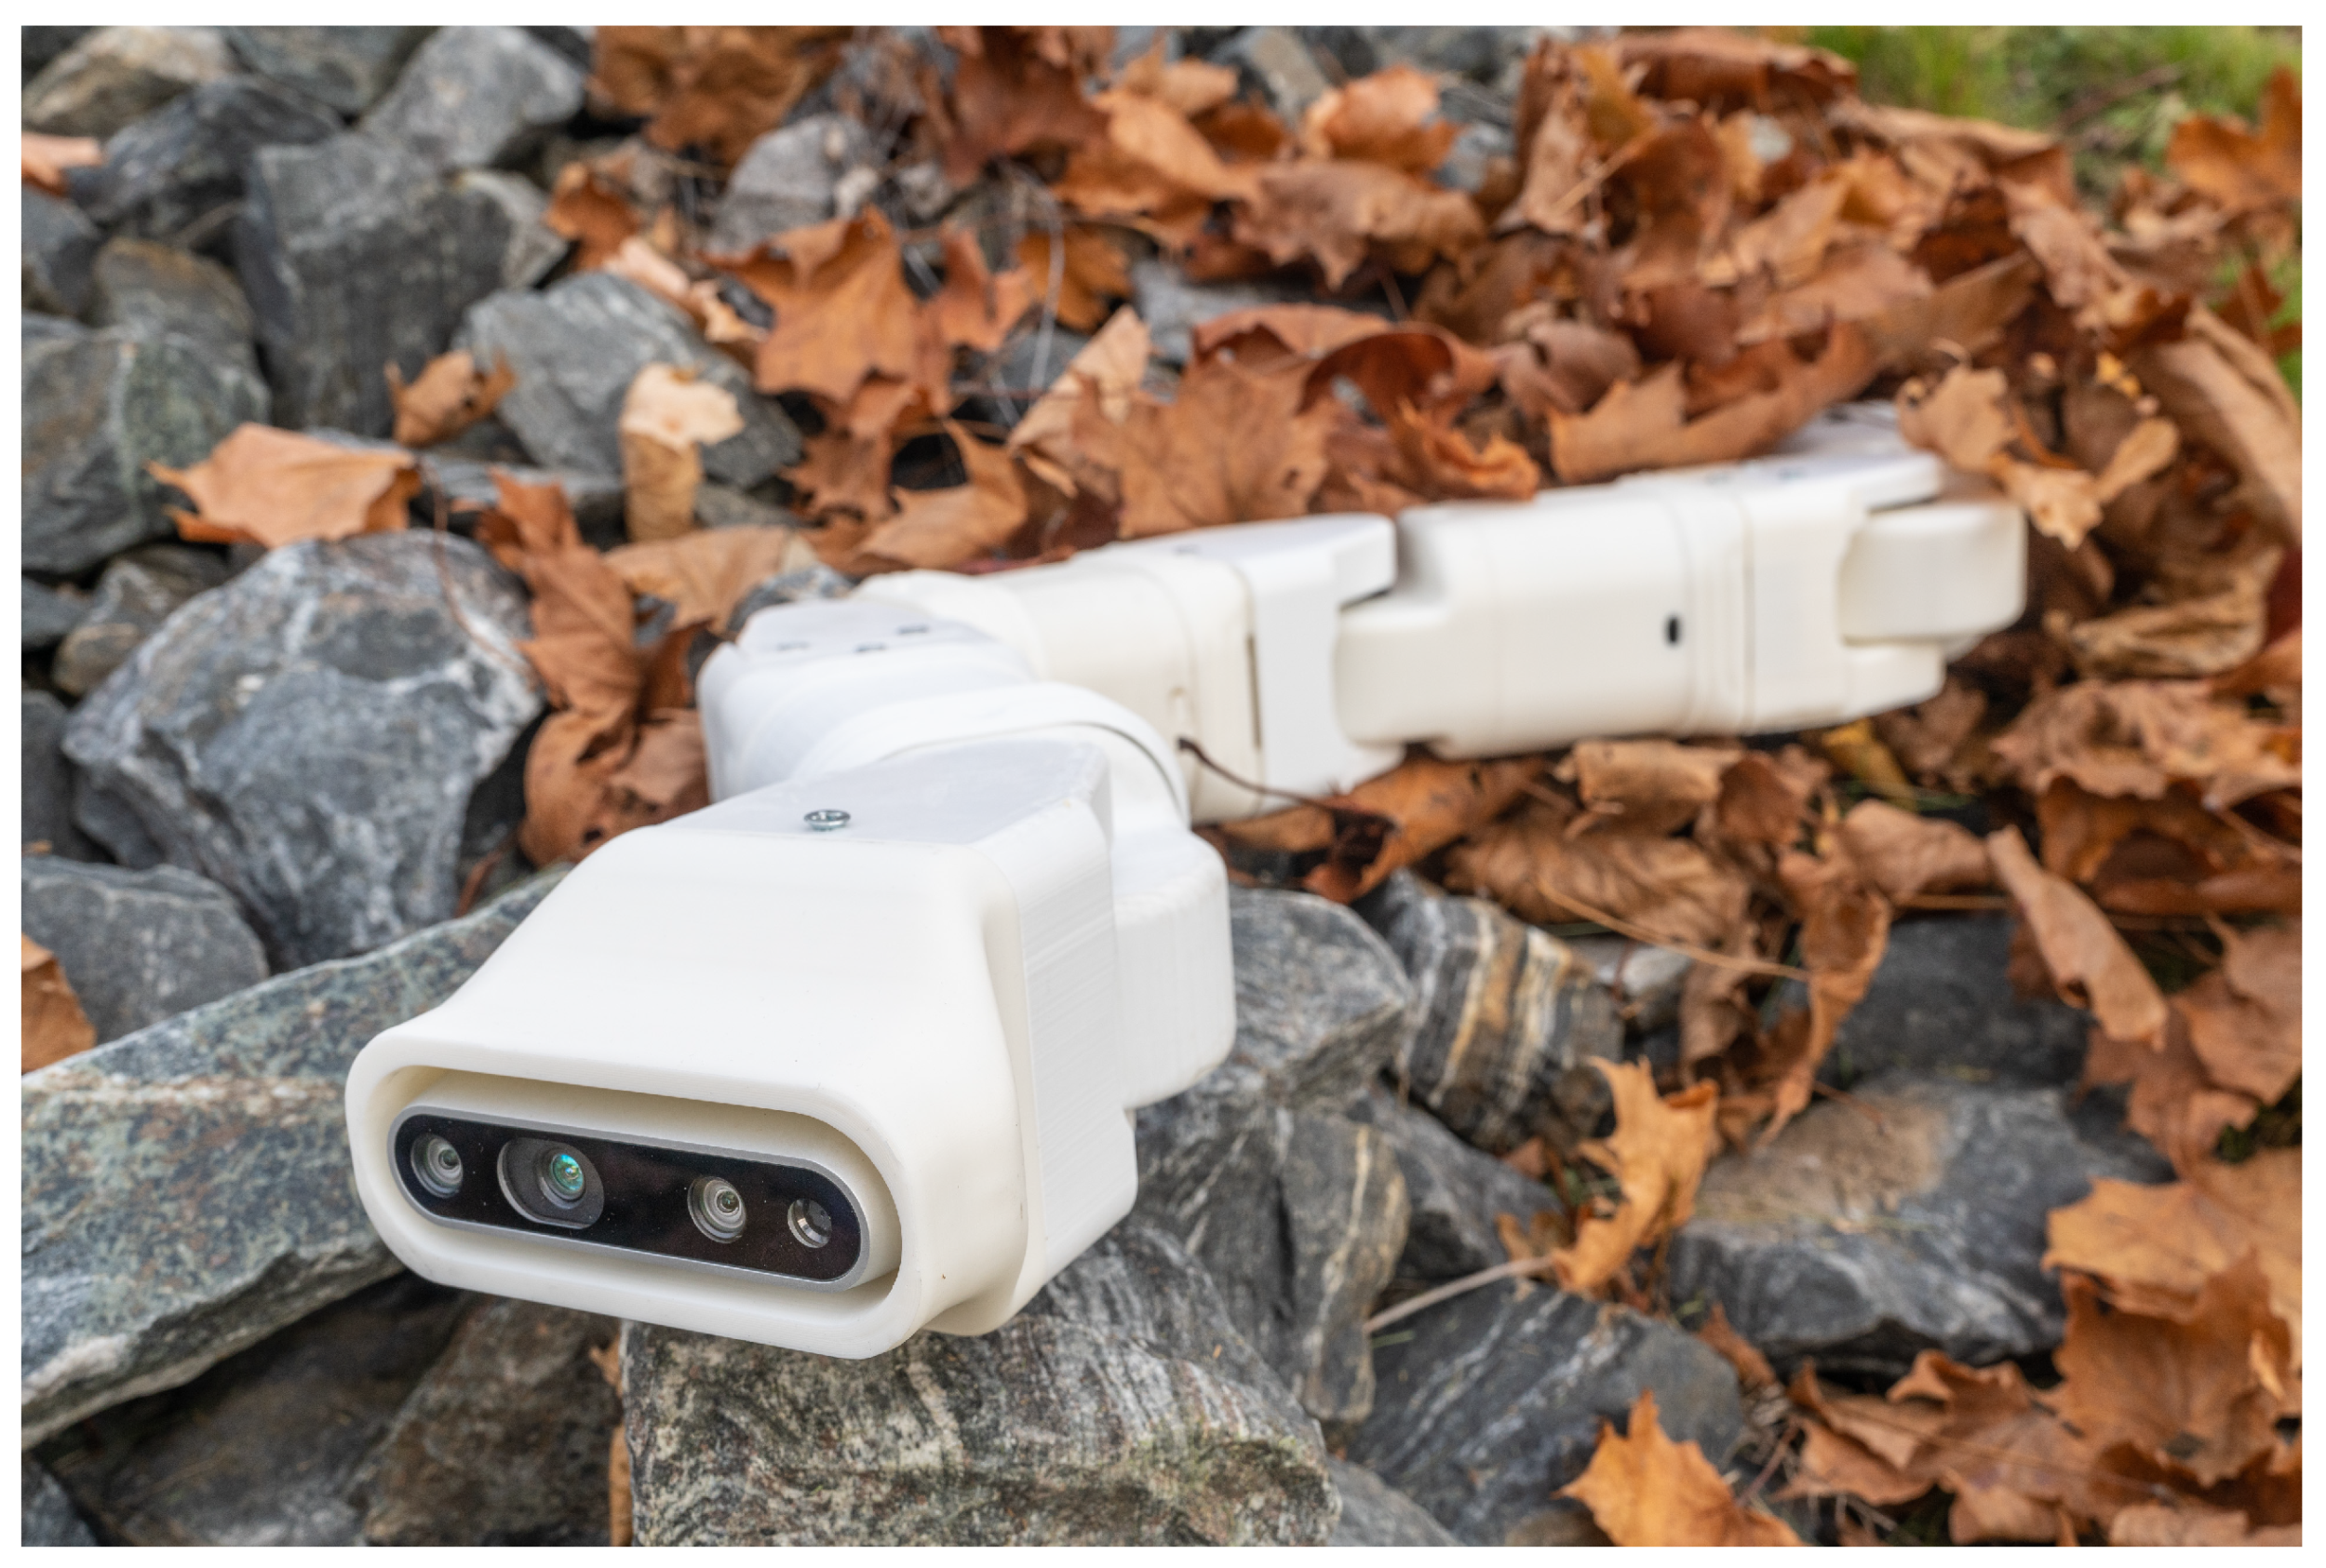
\includegraphics[scale=0.7]{figures/ros-snake.png}
\caption{ROS-based snake robot (from \cite{sanfilippo2019serpens})}
\label{fig:ros_snake}
\end{center}
\end{figure}
JdeRobot\footnote {\href{https://jderobot.org/Main_Page}{JdeRobot}} is an opensource toolkit which facilitates the development in the fields of robotics and computer vision. Mainly written in the C++ programming language it provides a programming environment based on distributed components which can work together in an asynchronous and concurrent way to build applications.

\section{Deep learning frameworks}
This project makes use of the deep learning potential for the object detection task and, for this reason, deep learning frameworks are needed. In particular, the following will be used: \textit{Tensorflow} and \textit{Keras}.\\
As introduced in section \ref{dl_frameworks}, Tensorflow is an open-source platform for machine learning and that includes deep learning. It is often seen in deployment environments due to its flexibility allowing for more complex optimizations that are necessary when working in the real world. Keras can run on top of Tensorflow and other backends such as Theano or CNTK. This framework is more focussed on prototyping and fast experimentation.\\
Both frameworks will be used as building blocks for the neural network module. The object detection models selected in this project are going to run over the Python API of Tensorflow and Keras. The first one is used to prepare the inputs to the neural network models and to get the outputs (object detections) from the Tensorflow pre-trained object detectors (see section \ref{tf_models}). The Tensorflow models are saved using the \textit{pb}\footnote{\href{https://developers.google.com/protocol-buffers/?hl=en}{Protocol Buffers}} format from Google. The Protocol Buffers (commonly known as \textit{protobufs}) define data structures in text files that can be loaded or saved using different programming languages. Keras is used to build an SSD-VGG object detection architecture (see section \ref{keras_models}) and obtain the object detections. This framework uses the \textit{HDF5}\footnote{\href{https://www.hdfgroup.org/solutions/hdf5/}{HDF5}} file format for the data management.\\
The Tensorflow version used in this project is the 1.12.0 and the Keras version running is the 2.1.1.

\section{dlib library}
Written in C++, dlib\footnote {\href{http://dlib.net/}{dlib}} is a general purpose cross-platform library that follows the idea of component-based software engineering, i.e.\ a set of independent software components. This toolkit contains machine learning algorithms and tools to solve real world problems in domains including robotics, embedded devices or mobile phones. For example, dlib has an interesting face landmark detector. Landmarks in the face are basically key points in the face that can help in tasks such as person recognition. In the automotive industry landmarks are widely used to perform interior monitoring, i.e.\ to monitor the driver status.
\\In this project, the dlib library is used to perform object tracking. A correlation filter carries out the tracking using scale pyramid representation to handle large-scale variations in tracking \cite{danelljan2014accurate}. The version used is the 19.17.0.
\begin{figure}[H]
\begin{center}
\includegraphics[scale=0.15]{figures/dlib.jpg}
\caption{Facial landmarks with dlib, from the pre-trained model iBUG300-W \cite{sagonas2016300}}
\label{fig:pyqt}
\end{center}
\end{figure}

\section{Object Detection Metrics} \label{metrics_tool}
To obtain the results or statistics from the project the \href{https://github.com/rafaelpadilla/Object-Detection-Metrics}{\textit{Object-Detection-Metrics}} tool has been used. This tool written in Python by Rafael Padilla (thanks for sharing) provides the metrics used in the Pascal VOC object detection challenge: Precision x Recall curve and Average Precision.\\
It offers a simple format to work with results from an object detection application. In this case, it was used to obtain results from an object tracking application. Apart from the metrics it has also options to control the IoU threshold or the bounding boxes format, among others.\\
For installation and how-to-use instructions please refer to his \href{https://github.com/rafaelpadilla/Object-Detection-Metrics}{GitHub repository}.
\section{NumPy and PyQt}
Apart from the commented libraries and tools used for the project the following two need to be mentioned.
\begin{itemize}
\item \textbf{NumPy}\\
NumPy is the fundamental Python package for scientific computing specially for working with N-dimensional arrays such as matrixes. Images are basically matrixes at the end so here comes the necessity of this package. The version used of NumPy is the 1.15.4.
\item \textbf{PyQt}\\
PyQt provides a Python interface to the Qt library. Qt is a group of C++ libraries and development tools which include functionality to create graphical user interfaces, networks or threads, among others. In this project, PyQt is used in the \textit{GUI} module allowing the visualization of the results and the user interaction. The PyQt version used is the PyQt5.
\begin{figure}[H]
\begin{center}
\includegraphics[scale=0.5]{figures/pyqt.png}
\caption{PyQt5 example: common widgets (from \cite{pyqt})}
\label{fig:pyqt}
\end{center}
\end{figure}
\end{itemize}
